%% 
%% Copyright 2007-2024 Elsevier Ltd
%% 
%% This file is part of the 'Elsarticle Bundle'.
%% ---------------------------------------------
%% 
%% It may be distributed under the conditions of the LaTeX Project Public
%% License, either version 1.3 of this license or (at your option) any
%% later version.  The latest version of this license is in
%%    http://www.latex-project.org/lppl.txt
%% and version 1.3 or later is part of all distributions of LaTeX
%% version 1999/12/01 or later.
%% 
%% The list of all files belonging to the 'Elsarticle Bundle' is
%% given in the file `manifest.txt'.
%% 
%% Template article for Elsevier's document class `elsarticle'
%% with harvard style bibliographic references

\documentclass[preprint,12pt,authoryear]{elsarticle}
\usepackage{graphicx}      % include this line if your document contains figures
\usepackage{hyperref}
\usepackage{natbib}        % required for bibliography
%\usepackage{amsfonts}
\usepackage{tabularx}
\usepackage{caption}
%\usepackage{amssymb}
\usepackage{amsmath}
\usepackage{mathtools}
\usepackage{siunitx}
\usepackage{subfigure}
\usepackage{algorithm}
%\usepackage{algpseudocode}
\usepackage{booktabs}
\usepackage{url}
\usepackage{cite}
\usepackage{amsmath,amssymb,amsfonts}
\usepackage{algorithmic}
\usepackage{graphicx}
\usepackage{textcomp}
\usepackage{xcolor}
\usepackage{float}
\def\BibTeX{{\rm B\kern-.05em{\sc i\kern-.025em b}\kern-.08em
    T\kern-.1667em\lower.7ex\hbox{E}\kern-.125emX}}

\DeclareMathOperator{\argmin}{arg\;min}
\DeclareMathOperator{\vol}{vol}
\DeclareMathOperator{\diag}{diag}
\newcommand{\ui}[2]{#1_{\text{#2}}}
\newcommand{\uis}[2]{#1^{\text{#2}}}
\newcommand{\lrp}[1]{\left( #1 \right)}
\newcommand{\uib}[2]{{\bf #1}_{\text #2}}
\newcommand{\Ts}{\ui{T}{s}}

%% NN controller commands
\newcommand{\cnn}{\ui{\mathcal{C}}{NN}}
\newcommand{\fddpg}{\ui{f}{E}}
\newcommand{\uddpg}{\ui{u}{E}}
\newcommand{\actor}{\ui{f}{ACT}}
\newcommand{\critic}{\ui{f}{CRIT}}
\newcommand{\thx}{\ui{\theta}{x}}
\newcommand{\thf}{\ui{\theta}{f}}
\newcommand{\ucorr}{\widetilde{u}}
\newcommand{\unn}{\ui{u}{nn}}
\newcommand{\uact}{\ui{u}{ACT}}
\newcommand{\corr}{\ui{\mathcal{C}}{C}}
\newcommand{\todo}[1]{{{\color{red} TODO: #1	}} }
\renewcommand{\mark}[1]{{{\color{green} #1	}} }
%\newcommand{\e}[1]{\cdot 10^{#1}}
%%-------------------------------------------------------
%% MACRO for tikz picture. DO NOT CHANGE ANYTHING !!!!!
\usepackage{tikz}
\usepackage{pgfkeys}
\usepackage{calc}
\usepackage{pgfplots}
\usetikzlibrary{arrows}
\usetikzlibrary{calc}
\usepgflibrary{arrows}
\usetikzlibrary{positioning}
\usetikzlibrary{intersections}
\pgfplotsset{compat=newest}
\usetikzlibrary{shapes.geometric}
\usetikzlibrary{decorations.pathreplacing}
\usetikzlibrary{patterns,decorations.pathmorphing,decorations.markings}
\usetikzlibrary{external}
\usetikzlibrary{plotmarks}
\usetikzlibrary{arrows.meta}
\usepgfplotslibrary{patchplots}
\usepackage{grffile}
\usepgfplotslibrary{fillbetween}
\usepackage{xfrac}
%\tikzexternalize
\newcommand{\R}{\mathbb{R}}
\newcommand{\includetikz}[1]{%
\tikzifexternalizing{%
\def\DOIT{1}%
}{%
\IfFileExists{#1.pdf}{%
\includegraphics[scale=1]{#1.pdf}%
\def\DOIT{0}%
}{%
\def\DOIT{1}%
}%
}%
%
\if1\DOIT
%	\tikzsetnextfilename{mypic_#1}%
\tikzsetnextfilename{#1}
%   \filemodCmp{#1.tikz}{external/#1.log}%
%  {\tikzset{external/force remake=true}\input{#1.tikz}}
\input{#1.tikz}
\fi
}

% defines lengths for figure plotting
\newlength\figureheight
\newlength\figurewidth
%%  End of TikZ Macros
%%-------------------------------------------------------
\begin{document}

\begin{frontmatter}

%% Title, authors and addresses

%% use the tnoteref command within \title for footnotes;
%% use the tnotetext command for theassociated footnote;
%% use the fnref command within \author or \affiliation for footnotes;
%% use the fntext command for theassociated footnote;
%% use the corref command within \author for corresponding author footnotes;
%% use the cortext command for theassociated footnote;
%% use the ead command for the email address,
%% and the form \ead[url] for the home page:
%% \title{Title\tnoteref{label1}}
%% \tnotetext[label1]{}
%% \author{Name\corref{cor1}\fnref{label2}}
%% \ead{email address}
%% \ead[url]{home page}
%% \fntext[label2]{}
%% \cortext[cor1]{}
%% \affiliation{organization={},
%%            addressline={}, 
%%            city={},
%%            postcode={}, 
%%            state={},
%%            country={}}
%% \fntext[label3]{}

\title{The Beggining of Control Revolution: Ofset-free Koopman MPC} %% Article title

%% use optional labels to link authors explicitly to addresses:
%% \author[label1,label2]{}
%% \affiliation[label1]{organization={},
%%             addressline={},
%%             city={},
%%             postcode={},
%%             state={},
%%             country={}}
%%
%% \affiliation[label2]{organization={},
%%             addressline={},
%%             city={},
%%             postcode={},
%%             state={},
%%             country={}}

\author{Patrik Valábek} %% Author name

%% Author affiliation
\affiliation{organization={STU},%Department and Organization
            addressline={Redlinskeho 9}, 
            city={Bratislava},
            country={Slovakia}}

%% Abstract
\begin{abstract}
%% Text of abstract

\end{abstract}

%%Graphical abstract
%\begin{graphicalabstract}
%\includegraphics{grabs}
%\end{graphicalabstract}

%%Research highlights
\begin{highlights}
\item Research highlight 1
\item Research highlight 2
\end{highlights}

%% Keywords
\begin{keyword}
%% keywords here, in the form: keyword \sep keyword

%% PACS codes here, in the form: \PACS code \sep code

%% MSC codes here, in the form: \MSC code \sep code
%% or \MSC[2008] code \sep code (2000 is the default)

\end{keyword}

\end{frontmatter}

%% Add \usepackage{lineno} before \begin{document} and uncomment 
%% following line to enable line numbers
%% \linenumbers

%% main text
%%
\section{Introduction}
\label{sec:intro}

\section{Preliminaries and Notation}
\label{sec:Preliminaries}

\subsection{Parsim-K Identification}
 
\subsection{Offset-Free MPC}

\subsection{Nonlinear MPC}

\subsection{Koopman Operator}

\subsection{Koopman MPC}

\subsection{State Estimation - Observer}

\section{Koopman MPC with Offset-Free - Easyiest}
In this section, we will present a standard offset free optimal framework consisting of Target Optimization, State Estimation - Observer and MPC. As observer is standard Kalman filter or extended Kalman filter, we will discuss mainly remaining two optimization problems. Both remaining components had to be designed in a way that they are able to work with the Koopman operator. The main goal of this section is to show that the standard formulation can be easily transformed for the offset-free MPC use.

\begin{figure}[H]
  \centering
  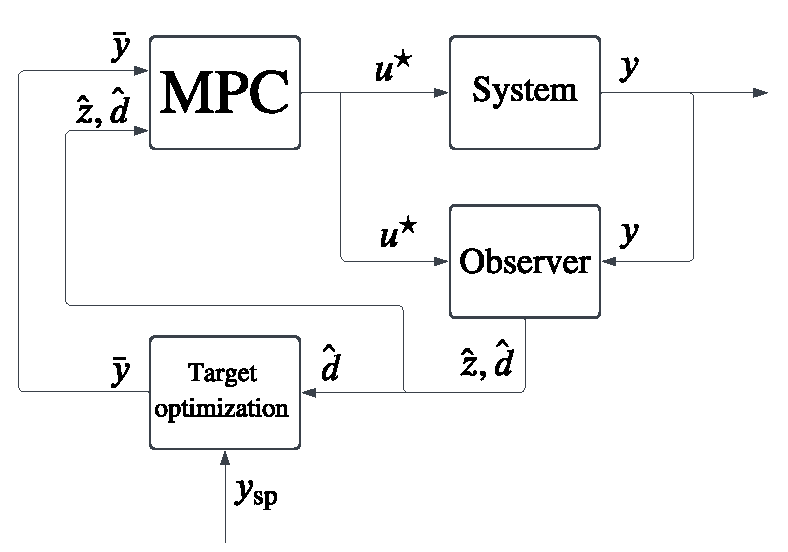
\includegraphics[width=0.95\linewidth]{figures/close_loop.pdf}
  \caption{Closed-loop control structure.}
  \label{fig:close_loop}
\end{figure}

\subsection{Target Optimization}

\begin{subequations}
  \label{eq:target:opt}
  \begin{align}
    \min_{\bar{u}, \bar{z}, \bar{y}} \quad & \; (\bar{y} - y_\text{ref})^\intercal Q_\text{y} (\bar{y} - y_\text{ref}) \label{eq:target:opt:obj} \\
    \text{s.t.} \quad & \; \bar{z} = A\bar{z} + B\bar{u} \label{eq:target:opt:z} \\
    & \; \bar{y} = C\bar{z} + d \label{eq:target:opt:y} \\
    & \; u_{\min} \leq \bar{u} \leq u_{\max} \label{eq:target:opt:u} \\
    & \; y_{\min} \leq \bar{y} \leq y_{\max} \label{eq:target:opt:ycon} \\
    & \; d = \hat{d}(t), \quad y_\text{ref} = y_\text{sp} \label{eq:target:opt:params}
  \end{align}
\end{subequations}



\subsection{MPC}
\begin{subequations}
  \label{eq:of:mpc}
  \begin{align}
    \min_{u_0, \ldots, u_{N-1}} \; & \; \sum_{k=0}^{N-1} (y_k - \bar{y})^\intercal Q_\text{y} (y_k - \bar{y}) + \sum_{k=0}^{N-1} \Delta u_k^\intercal Q_\text{u} \Delta u_k, \label{eq:of:mpc:obj} \\
    \text{s.t.} \;\;\;\; & \; z_{k+1} = A z_k + B u_k, \quad k\in\mathbb{N}_0^{N-1}, \label{eq:of:mpc:z} \\
    & \; y_k = C z_k + d, \quad k\in\mathbb{N}_0^{N-1}, \label{eq:of:mpc:y} \\
    & \; \Delta u_k = u_k - u_{k-1}, \quad k\in\mathbb{N}_0^{N-1}, \label{eq:of:mpc:du} \\
    & \; u_{\min} \leq u_k \leq u_{\max}, \quad k\in\mathbb{N}_0^{N-1}, \label{eq:of:mpc:u} \\
    & \; y_{\min} \leq y_k \leq y_{\max}, \quad k\in\mathbb{N}_0^{N-1}, \label{eq:of:mpc:ycon} \\
    & \; z_0 = \hat{z}(t), \quad d = \hat{d}(t), \quad u_{-1} = u(t-T_\text{s}) \label{eq:of:mpc:init}
  \end{align}
\end{subequations}

\section{Koopman MPC with Offset-Free - Proposed}

Main drawback that we observe in a current Koopman MPC (offset-free, robust, or any other), is that the optimization is done without leveraging knowledge of the lifted space. Of course we are predicting in the lifted space, but in objective function we are using original space, that is created derived as linear transformation of the lifted space. This transformation is not linear by nature, but to use linear MPC, we think we had no other choice. Some papers are not using this transformation directly, but after closer look, they are usualy using equivalent transformations. We will show that we can use the lifted space directly in the objective function, show how to handle the lifted space and transformation of an objective function.
We can fully eliminate the neccessity of the back transformation used in objective function in MPC, but we still need them to compute the target for the lifted space. In this case and case of constraints, we use a first order Taylor expansion, to better approximate the transformation. 

\subsection{Target Optimization}
\begin{subequations}
  \label{eq:cs:target}
  \begin{align}
    \min_{\bar{u}, \bar{z}} \quad & \; (\bar{y} - y_\text{ref})^\intercal Q_\text{y} (\bar{y} - y_\text{ref}) \label{eq:cs:target:obj} \\
    \text{s.t.} \quad & \; \bar{z} = A\bar{z} + B\bar{u} \label{eq:cs:target:z} \\
    & \; \bar{y} = H(z_k)\bar{z} + h(z_k) - H(z_k)z_k + d \label{eq:cs:target:y} \\
    & \; u_{\min} \leq \bar{u} \leq u_{\max} \label{eq:cs:target:u} \\
    & \; y_{\min} \leq \bar{y} \leq y_{\max} \label{eq:cs:target:ycon} \\
    & \; d = \hat{d}(t), \quad y_\text{ref} = y_\text{sp}, \quad z_k = \hat{z}(t) \label{eq:cs:target:params}
  \end{align}
\end{subequations}

\subsection{MPC}
\begin{subequations}
  \label{eq:cs:mpc}
  \begin{align}
    \min_{u_0, \ldots, u_{N-1}} \; & \; \sum_{k=0}^{N-1} (z_k - \bar{z})^\intercal Q_\text{z} (z_k - \bar{z}) + \sum_{k=0}^{N-1} \Delta u_k^\intercal Q_\text{u} \Delta u_k, \label{eq:cs:mpc:obj} \\
    \text{s.t.}\;\;\;\; & \; z_{k+1} = A z_k + B u_k, \quad k\in\mathbb{N}_0^{N-1}, \label{eq:cs:mpc:z} \\
    & \; y_k = H(z_0) z_k + h(z_0) - H(z_0)z_0 + d, \quad k\in\mathbb{N}_0^{N-1}, \label{eq:cs:mpc:y} \\
    & \; \Delta u_k = u_k - u_{k-1}, \quad k\in\mathbb{N}_0^{N-1}, \label{eq:cs:mpc:du} \\
    & \; u_{\min} \leq u_k \leq u_{\max}, \quad k\in\mathbb{N}_0^{N-1}, \label{eq:cs:mpc:u} \\
    & \; y_{\min} \leq y_k \leq y_{\max}, \quad k\in\mathbb{N}_0^{N-1}, \label{eq:cs:mpc:ycon} \\
    & \; z_0 = \hat{z}(t), \quad d = \hat{d}(t), \quad u_{-1} = u(t-T_\text{s}) \label{eq:cs:mpc:init}
  \end{align}
\end{subequations}

\section{Block Diagonal Deep Koopman Transformation}

\begin{table}[h]
  \centering
  \caption{Comparison of structure of A}
  \label{tab:ident-comp}
  \begin{tabular}{cccccc}
      \toprule
        Structure & Time TE/MPC & Optimal? \([\%]\) & OBJ & ST \(h_1\) & ST \(h_2\) \\
        \midrule
        Full          & 0.2392 / 2.3884 & 26.7 & 100.0 & 43 & 48 \\
        Block Diagonal & 0.2191 / 1.6204 & 100.0 & 94.1 & 25 & 31 \\
        \bottomrule
  \end{tabular}
\end{table}

\section{Simulation Setup}

\section{Simulation Results}
\label{sec:Results}

% \begin{table}[h]
%   \centering
%   \caption{Comparison of several methods}
%   \label{tab:ident-comp}
%   \begin{tabular}{cccccc}
%       \toprule
%         Structure & OBJ u  & OBJ y & OBJ & ST \(h_1\) & ST \(h_2\) \\
%         \midrule
%         NMPC          & 4.4568 & 20.3818 & 100.0  & 8 & 8 \\%(24.8386)
%         Parsim-K      & 6.0253 & 24.5910 & 123.3 & 27 & 27 \\
%         Full C          & 3.8177 & 23.8167 & 111.3 & 66 & 78 \\
%         Block Diagonal C & 3.8492 & 22.4462 & 105.9 & 47 & 42 \\
%         Full \(C_k\)          & 11.5966 & 18.9656 & 123.0 & 31 & 23 \\
%         Block Diagonal \(C_k\) &  11.5214 & 19.0154 & 122.9 & 30 & 23 \\
%         \bottomrule
%   \end{tabular}
% \end{table}
\begin{table}[h]
  \centering
  \caption{Comparison of several Tunings}
  \label{tab:ident-comp}
  \begin{tabular}{cccc}
      \toprule
        LP MPC & LP TE & Tuning & OBJ \\
        \midrule
        - & - & \(J(z_s)\)          & 171.22 \\%(24.8386)
        \(C\) & \(C\) & \(J(z_s)\)           & 147.26 \\
        \(J(z_s)\) \text{w/o y-con} & \(J(z_{s,k-1})\) & \(J(z_s)\)           & 149.18 \\ 
        \(J(z_k)\) & \(J(z_k)\) & \(J(z_s)\)          & 163.69 \\
        \(J(z_k)\) & \(J(z_s)\) & \(J(z_s)\)          & 149.35 \\
        \midrule
        - & - & \(C\)          & 156.21 \\%(24.8386)
        \(C\) & \(C\) & \(C\)            & 151.73 \\
        \(J(z_s)\) \text{w/o y-con} & \(J(z_{s,k-1})\) & \(C\)            & 158.80 \\ 
        \(J(z_k)\) & \(J(z_k)\) & \(C\)           & 177.33 \\
        \(J(z_k)\) & \(J(z_s)\) & \(C\)           & 158.68 \\
        \bottomrule
  \end{tabular}
\end{table}

\begin{table}[h]
  \centering
  \caption{Comparison of several Tunings}
  \label{tab:ident-comp}
  \begin{tabular}{cccc}
      \toprule
        ALG & MODEL & OBJ \\
        \midrule
        NMPC & Tru & 88.09  \\%(24.8386)
        MPC & Pa.-K (3) & 167.51  \\
        MPC & DK & 156.21  \\
        TMPC & DK (C) & 147.22  \\
        TMPC & DK (J(z)) & 149.35  \\
        \bottomrule
  \end{tabular}
\end{table}

%\bibliographystyle{elsarticle-num-names}  % Elsevier's numbered citation style
%\bibliography{bibfile}
 % Reference your .bib file (without .bib extension)
\end{document}
 
\endinput
%%
%% End of file `elsarticle-template-harv.tex'.


